\documentclass{beamer}
\usepackage{xcolor} 
\usepackage[utf8]{inputenc}
\usetheme{Madrid}
\usecolortheme{beaver}

%Information to be included in the title page:
\title[About Beamer] %optional
{Software for embedded systems}

\subtitle{Verification Lab.\\ (Assertion-based verification)}

\author{Alessandro Danese}
\institute{University of Verona, Verona, Italy
\\alessandro.danese@univr.it}
%\date{2019}
 
 
\begin{document}
 
\frame{\titlepage}
 
%==================================================================================
\begin{frame}
\frametitle{Simple-platform case study}

How to download the simple platform:
\begin{block}{}
	git clone https://AlessandroDanese@bitbucket.org/AlessandroDanese/sse-verifica.git
\end{block}

How to open the simple platform-project case study:
\begin{block}{}
\begin{enumerate}
	\item 
	open Vivado
	\item
	File -$>$ Open project... -$>$ path2/sse-verifica/simple-platform/simple\_platform.xpr
\end{enumerate}
\end{block}

\end{frame}
%----------------------------------------------------------------------------------
 
%==================================================================================
\begin{frame}
\frametitle{Vivado}
Once started, the following window should appear

\begin{figure}
	\centering
	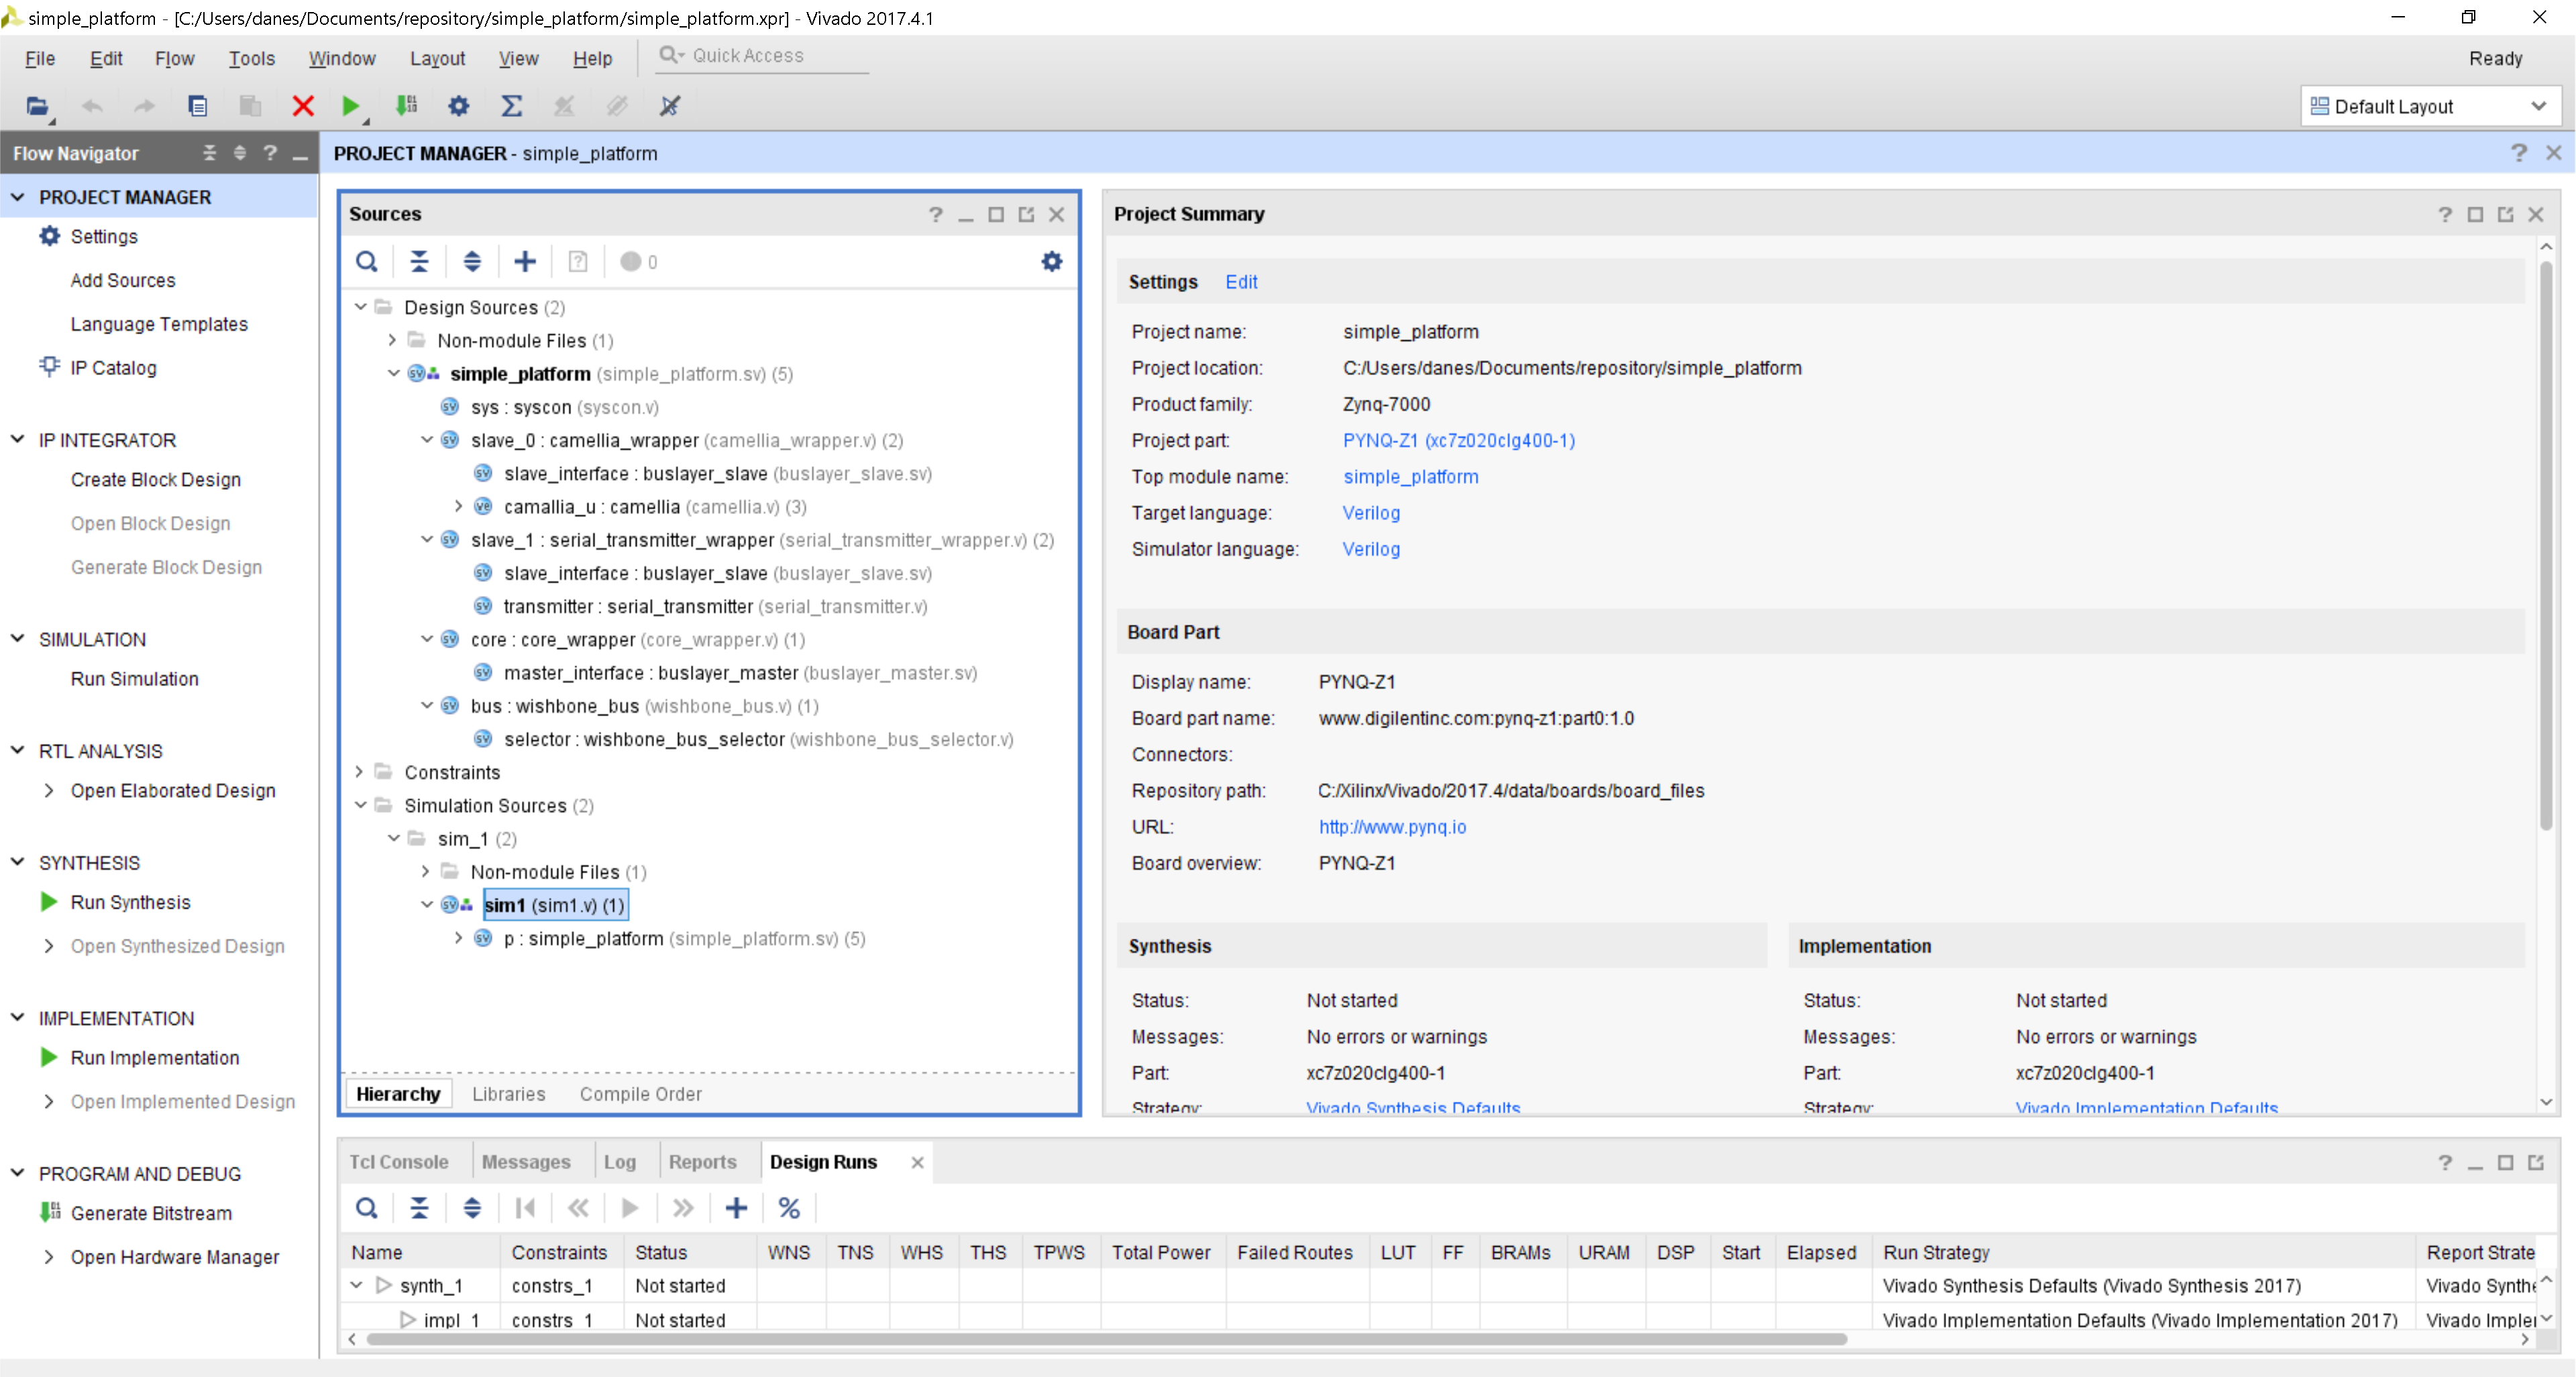
\includegraphics[width=0.9\columnwidth]{figures/vivado_sp.png}
\end{figure}

\end{frame}
%----------------------------------------------------------------------------------

%==================================================================================
\begin{frame}
\frametitle{EDA tools}

How to download EDA tools:

\begin{block}{}
\begin{enumerate}
	\item
	scp esd-student@esd-srv01.scienze.univr.it:/tmp/esdlab.tar.gz\\
	(password: esd-student)
	\item
	tar -xvf esdlab.tar.gz
	\item
	cd esdlab
	\item
	source start\_eda.bash
\end{enumerate}
\end{block}

\end{frame}
%----------------------------------------------------------------------------------


%==================================================================================
\begin{frame}

\frametitle{Makefile menu}
How to open the Makefile menu (terminal):
\begin{block}{}
	\begin{enumerate}
		\item 
		cd path2/sse-verifica/simple-platform/questa.simulation
		\item
		make
	\end{enumerate}
\end{block}

\end{frame}
%----------------------------------------------------------------------------------


%==================================================================================
\begin{frame}

\frametitle{Makefile menu}
Once started, the following menu should appear on the terminal

\begin{figure}
	\centering
	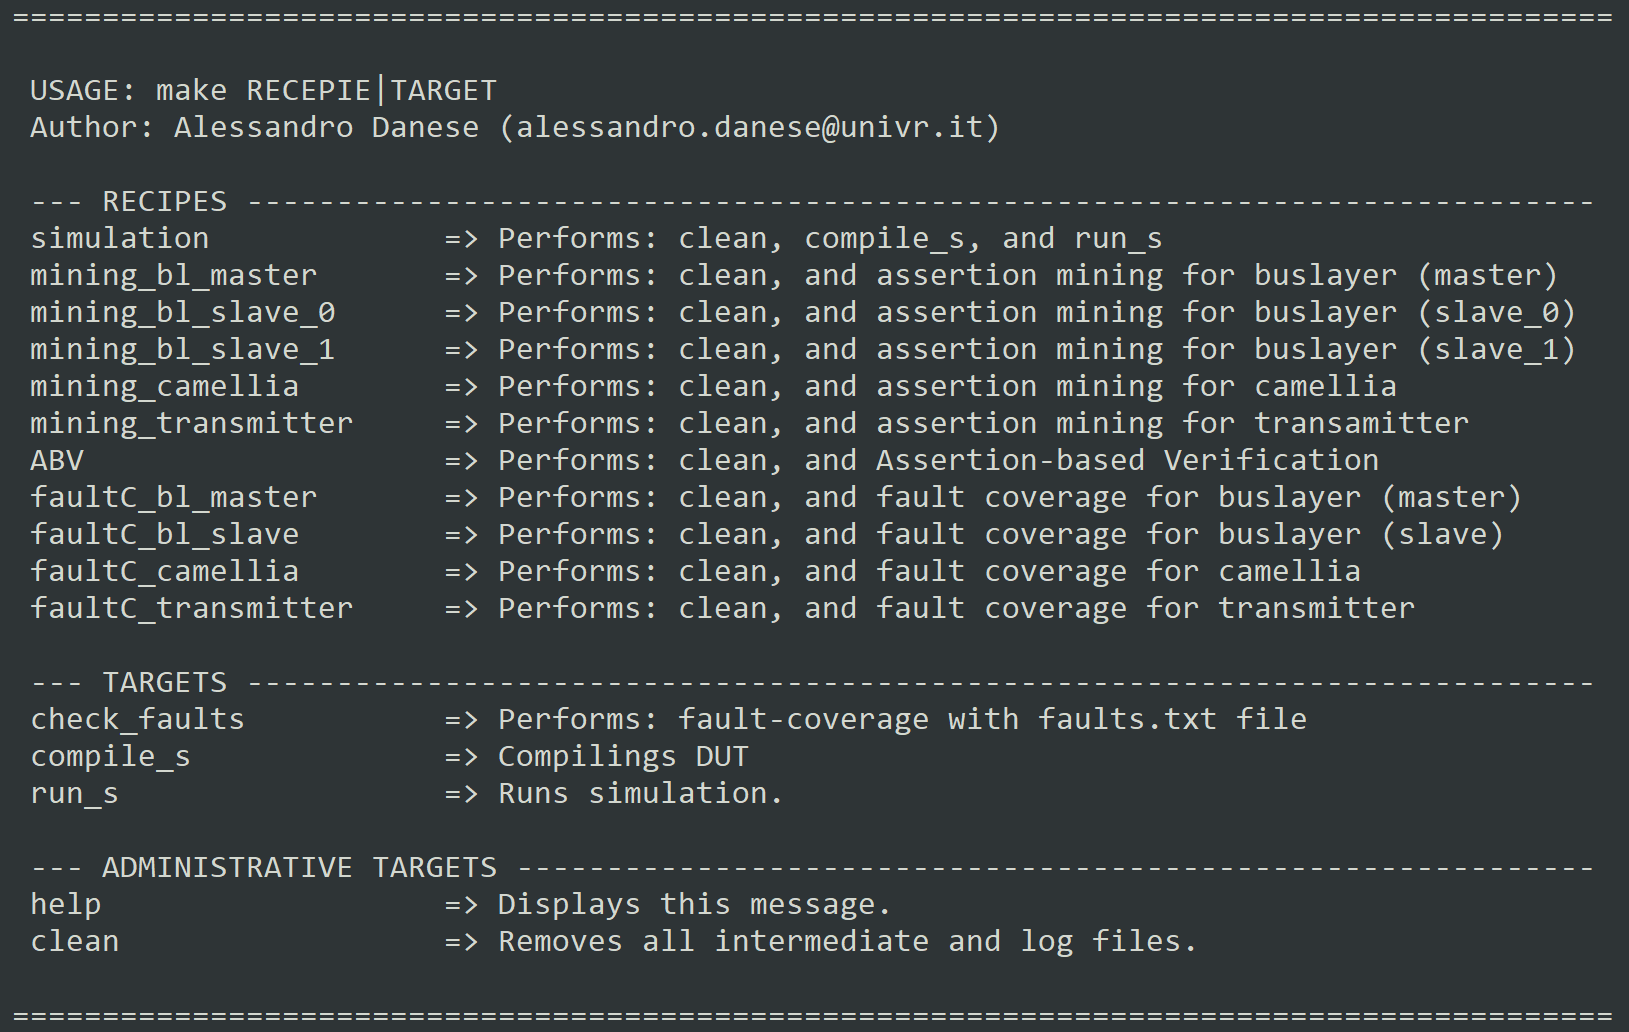
\includegraphics[width=0.9\columnwidth]{figures/makefile_menu.png}
\end{figure}
\end{frame}
%----------------------------------------------------------------------------------

%==================================================================================
\begin{frame}

\frametitle{Simulating the simple platform}

How to simulate the simple platform
\begin{block}{}
	\begin{enumerate}
		\item
		make simulation
	\end{enumerate}
\end{block}

The command \textit{make simulation} compiles the platform and the firmware 
source code (directory firmware).\\~\\ Afterwards, it runs a simulation.

The sim.vcd file records the values of any register/wire/port of the platform.
The transactor\_log.txt file records any read\_transaction and write\_transaction performed by the firmware. 

\end{frame}
%----------------------------------------------------------------------------------

%==================================================================================
\begin{frame}

\frametitle{Assertion-based verification (ABV)}

How to perform ABV with the simple platform
\begin{block}{}
	\begin{enumerate}
		\item
		make ABV
	\end{enumerate}
\end{block}

The command \textit{make ABV} compiles the source code of the platform,
the firmware source code, and the verification unit in the files:
buslayer\_master.psl, buslayer\_slave.psl, camellia.psl and transmitter.psl
(sse\_lesson1/vcs.simulation/psl).

\end{frame}
%----------------------------------------------------------------------------------

%==================================================================================
\begin{frame}

\frametitle{Verification unit}

A verification \textbf{vunit} is used to group PSL directives, and modeling code.
A vunit is written in a side file that is bound to all the specified component's 
instances during the simulation.
\begin{block}{}
	vunit (component\_name) \{\\
	...\\
	\}
\end{block}

Advantage:\\
\begin{itemize}
	\item 
	we do not change the source code of the component
	\item
	no glue logic to bind component's instances and properties
	\item
	properties and component's instances are connected automatically
	\item
	assertion failures are notified automatically 
\end{itemize}

\end{frame}
%----------------------------------------------------------------------------------


%==================================================================================
\begin{frame}

\frametitle{PSL directive}

\begin{block}{directive template}
formula = [StrId:] directive (Property [@ clock]) [report Str];\\
directive = assert $|$ cover $|$ ...
\end{block}

\end{frame}
%----------------------------------------------------------------------------------

%==================================================================================
\begin{frame}

\frametitle{Sampled value}
\textbf{The sampled value is the only valid value of a variable in a Property!}\\~\\
The sampled value is the value of a variable before a clock tick.
A clock tick is an atomic moment in time that itself spans no duration of time.

\begin{figure}
\centering
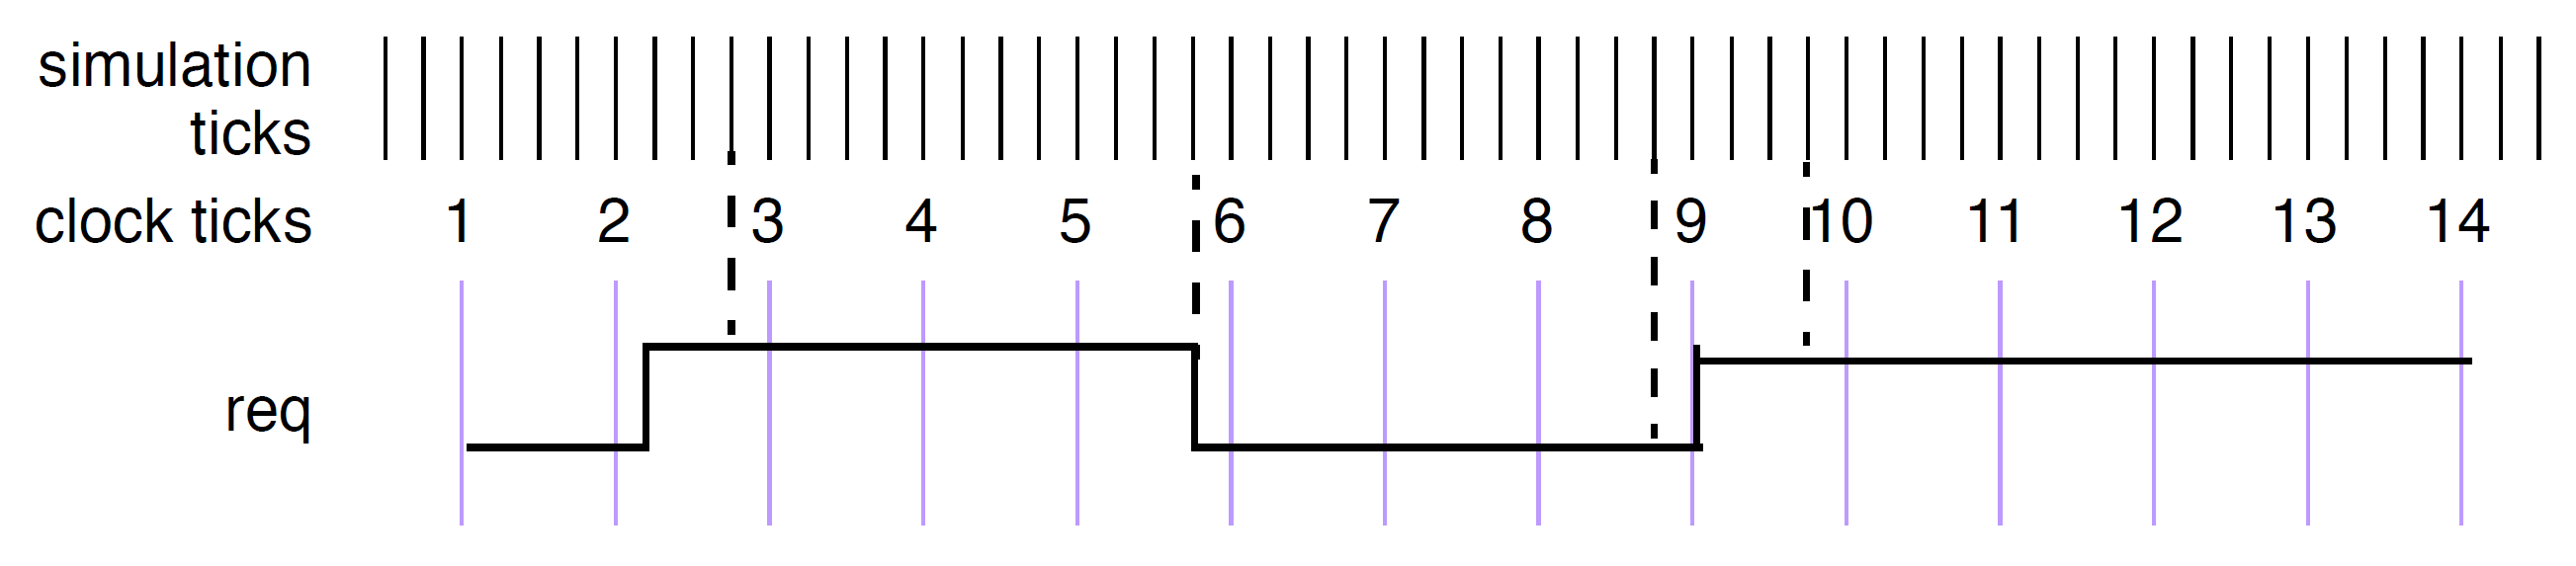
\includegraphics[width=0.9\columnwidth]{figures/sampled_value.png}
\end{figure}

req is high at clock ticks: 3, 4, 5, 10, 11, 12, 13, 14.\\
At 9th clock tick, req is still low!\\~\\

\end{frame}
%----------------------------------------------------------------------------------

%==================================================================================
\begin{frame}

\frametitle{Exercise - 1}

Each file doc/*\_spec.pdf contains a description of the functionality
of the platform's components in natural language.\\~\\

The current implementation of the simple platform does not meet all the 
listed specifications!\\~\\

As a verification engineer, you are required to formalize the specifications
of the platform's components in PSL, and find all the bugs!   
 
\end{frame}
%----------------------------------------------------------------------------------

%==================================================================================
\begin{frame}

\frametitle{Exercise - 2}

As a verification engineer, you are required to formalize the behaviour of the 
component transmitter.\\~\\
The transmitter component has not got a document describing its functionality. In
this case, its behaviour can be inferred from its simulation trace, the mined 
assertions and from the source code.

\end{frame}
%----------------------------------------------------------------------------------


\end{document}